% OWNER: P1 (lead). Numbers ONLY via macros from generated/numbers.tex (regenerate: python paper/tools/make_numbers.py).
% Source of truth: eval/tier2_entity_runs/TIER2_FULL_entity_report_v1.json (sha256 18b5d9df...), regenerated byte-for-byte by
% python -m tier2.entity_report_verified. If the review produces exclusions, ADD the sensitivity table; never replace the primary one.
\section{Results}
\label{sec:results}

All results are from one seed with greedy decoding, on development data, with 95\% Wilson intervals; paired contrasts use a percentile
bootstrap over pairs and the exact McNemar test. We report two settings on the \emph{same} 63 in-scope Hindi source pairs (36
gold-different, 27 gold-same): Tier~1 compares each pair in isolation with a 3B backbone (all four configurations), and Tier~2 injects the
pair into a six-session conversation with distractors and a 7B judge (Configs C and D).

\subsection{Tier 1: isolated pairs, Configurations A--D}

\begin{table}[t]\centering\small
\resizebox{\linewidth}{!}{% GENERATED by paper/tools/make_tier1_numbers.py. Do not edit.
\begin{tabular}{llcccc}
\toprule
Config & DK-Mem & FCR (in-scope hi) & MCR (in-scope hi) & FCR (all) & MCR (all) \\
\midrule
A & gate off & 7/36 [0.10, 0.35] & 0/27 [0.00, 0.12] & 29/98 [0.21, 0.39] & 19/75 [0.17, 0.36] \\
A & gate on & 0/36 [0.00, 0.10] & 5/27 [0.08, 0.37] & 22/98 [0.15, 0.32] & 24/75 [0.23, 0.43] \\
A & gate on + LLM fallback & 0/36 [0.00, 0.10] & 5/27 [0.08, 0.37] & 22/98 [0.15, 0.32] & 24/75 [0.23, 0.43] \\
\midrule
B & gate off & 1/36 [0.00, 0.14] & 6/27 [0.11, 0.41] & 40/98 [0.32, 0.51] & 27/75 [0.26, 0.47] \\
B & gate on & 1/36 [0.00, 0.14] & 8/27 [0.16, 0.48] & 40/98 [0.32, 0.51] & 29/75 [0.28, 0.50] \\
B & gate on + LLM fallback & 1/36 [0.00, 0.14] & 8/27 [0.16, 0.48] & 40/98 [0.32, 0.51] & 29/75 [0.28, 0.50] \\
\midrule
C & gate off & 0/36 [0.00, 0.10] & 1/27 [0.01, 0.18] & 45/98 [0.36, 0.56] & 22/75 [0.20, 0.40] \\
C & gate on & 0/36 [0.00, 0.10] & 6/27 [0.11, 0.41] & 45/98 [0.36, 0.56] & 27/75 [0.26, 0.47] \\
C & gate on + LLM fallback & 0/36 [0.00, 0.10] & 6/27 [0.11, 0.41] & 45/98 [0.36, 0.56] & 27/75 [0.26, 0.47] \\
\midrule
D ($\tau$=0.90) & gate off & 24/36 [0.50, 0.80] & 11/27 [0.25, 0.59] & 44/98 [0.35, 0.55] & 38/75 [0.40, 0.62] \\
D ($\tau$=0.90) & gate on & 0/36 [0.00, 0.10] & 11/27 [0.25, 0.59] & 20/98 [0.14, 0.29] & 38/75 [0.40, 0.62] \\
D ($\tau$=0.90) & gate on + LLM fallback & 0/36 [0.00, 0.10] & 11/27 [0.25, 0.59] & 20/98 [0.14, 0.29] & 38/75 [0.40, 0.62] \\
\midrule
D ($\tau$=0.85) & gate off & 32/36 [0.75, 0.96] & 4/27 [0.06, 0.32] & 70/98 [0.62, 0.79] & 30/75 [0.30, 0.51] \\
D ($\tau$=0.85) & gate on & 1/36 [0.00, 0.14] & 7/27 [0.13, 0.45] & 39/98 [0.31, 0.50] & 33/75 [0.33, 0.55] \\
D ($\tau$=0.85) & gate on + LLM fallback & 1/36 [0.00, 0.14] & 7/27 [0.13, 0.45] & 39/98 [0.31, 0.50] & 33/75 [0.33, 0.55] \\
\midrule
D ($\tau$=0.80) & gate off & 35/36 [0.86, 1.00] & 2/27 [0.02, 0.23] & 94/98 [0.90, 0.98] & 21/75 [0.19, 0.39] \\
D ($\tau$=0.80) & gate on & 3/36 [0.03, 0.22] & 6/27 [0.11, 0.41] & 62/98 [0.53, 0.72] & 25/75 [0.24, 0.45] \\
D ($\tau$=0.80) & gate on + LLM fallback & 3/36 [0.03, 0.22] & 6/27 [0.11, 0.41] & 62/98 [0.53, 0.72] & 25/75 [0.24, 0.45] \\
\bottomrule
\end{tabular}
}
\caption{Tier~1 (Qwen2.5-3B, seed 0; labels LLM-annotated, provisional). ``In-scope hi'': kinship, honorific register and name-variant
pairs in Hindi, the source pairs of Tier~2. ``All'': all 173 pairs (Hindi, Korean, Turkish, German), including classes the lexicon does
not cover. The LLM fallback equals the plain gate here because the Hindi lexicon flags no class as ambiguous on these items.}
\label{tab:tier1}
\end{table}

\paragraph{The gate removes almost all false merges of the embedding host.} For Config D at $\tau=0.90$, in-scope Hindi FCR falls from
\TOneDNinetyOffHiFCR{} to \TOneDNinetyLexHiFCR{} with MCR unchanged (\TOneDNinetyOffHiMCR{}); at $\tau=0.85$ from \TOneDEightyFiveOffHiFCR{}
to \TOneDEightyFiveLexHiFCR{}. For Config A, from \TOneAOffHiFCR{} to \TOneALexHiFCR{} (MCR \TOneAOffHiMCR{} $\to$ \TOneALexHiMCR{}).
For Config C, the 3B judge already makes no in-scope Hindi false merge (\TOneCOffHiFCR{}), so the gate can only add missed merges
(\TOneCOffHiMCR{} $\to$ \TOneCLexHiMCR{}). For B, false merges stay at \TOneBOffHiFCR{} and missed merges rise from \TOneBOffHiMCR{}
to \TOneBLexHiMCR{}. Over all 173 pairs the gate leaves the false merges of B and C unchanged (\TOneBOffAllFCR{} and
\TOneCOffAllFCR{}), because most of them fall in languages and classes the Hindi lexicon does not cover. A judge that under-merges
gains nothing from a veto-only gate; in Tier~2 the 7B judge over-merges, and there the gate helps (Section~\ref{sec:results-v2}).

\subsection{Tier 2: multi-session conversations, Configurations C and D}

\begin{table}[t]\centering\small
% GENERATED by paper/tools/make_numbers.py. Do not edit.
\begin{tabular}{llcccc}
\toprule
Arm & Run & FCR (all) & MCR (all) & FCR (Hindi) & MCR (Hindi) \\
\midrule
Main & C, gate off & 15/42 [0.23, 0.51] & 0/27 [0.00, 0.12] & 9/36 [0.14, 0.41] & 0/27 [0.00, 0.12] \\
Main & C, gate on & 7/42 [0.08, 0.31] & 5/27 [0.08, 0.37] & 1/36 [0.00, 0.14] & 5/27 [0.08, 0.37] \\
Main & D, gate off & 5/42 [0.05, 0.25] & 27/27 [0.88, 1.00] & 0/36 [0.00, 0.10] & 27/27 [0.88, 1.00] \\
Main & D, gate on & 5/42 [0.05, 0.25] & 27/27 [0.88, 1.00] & 0/36 [0.00, 0.10] & 27/27 [0.88, 1.00] \\
\midrule
Mirror & C, gate off & 11/42 [0.15, 0.41] & 1/27 [0.01, 0.18] & 5/36 [0.06, 0.29] & 1/27 [0.01, 0.18] \\
Mirror & C, gate on & 9/42 [0.12, 0.36] & 6/27 [0.11, 0.41] & 3/36 [0.03, 0.22] & 6/27 [0.11, 0.41] \\
Mirror & D, gate off & 0/42 [0.00, 0.08] & 27/27 [0.88, 1.00] & 0/36 [0.00, 0.10] & 27/27 [0.88, 1.00] \\
Mirror & D, gate on & 0/42 [0.00, 0.08] & 27/27 [0.88, 1.00] & 0/36 [0.00, 0.10] & 27/27 [0.88, 1.00] \\
\bottomrule
\end{tabular}

\caption{False consolidation rate (FCR, gold-different pairs merged) and missed consolidation rate (MCR, gold-same pairs not merged); lower
is better. ``All'' includes 6 German honorific pairs; ``Hindi'' excludes them. Main = v1.0 arm, Mirror = v1.1m counter-confound arm.}
\label{tab:results}
\end{table}

\paragraph{The LLM-judge host over-merges; the gate removes most false merges.} With the gate off, Config C merges \MainCoffHiFCR{} Hindi
gold-different pairs (\MainCoffHiFCRpct\%). With the gate, \MainClexHiFCR{}. Over all pairs, the gate changes the gold-different merge rate
by \MainCgateDiff{} (95\% CI \MainCgateDiffci{}; discordant pairs \MainCgateDiscordant{}, exact McNemar $p=\MainCgateMcNemar$).
The cost is missed merges: MCR rises from \MainCoffHiMCR{} to \MainClexHiMCR{}. \todo{P1: one sentence on why (underdetermined vetoes
when one side carries a kinship/register marker and the other does not).}

\paragraph{The embedding host does not separate the relations.} At $\tau=0.90$ Config D merges no gold-same pair (MCR \MainDoffHiMCR{}).
Its false merges (\MainDoffFCR{} over all pairs, \MainDoffHiFCR{} on Hindi) are all German. Figure~\ref{fig:dcos} shows why a single
threshold cannot work well here: in the Main arm, gold-different pairs share a sentence frame and so have \emph{higher} cosine (median
\MainDiffMedian{}, range \MainDiffMin{}--\MainDiffMax{}) than gold-same pairs, which carry different facts (median \MainSameMedian{},
\MainSameMin{}--\MainSameMax{}); \MainDiffAboveTau{} gold-different pairs exceed 0.90. In the Mirror arm the relation reverses
(gold-same median \MirrorSameMedian{} versus gold-different \MirrorDiffMedian{}). The ordering therefore follows how the benchmark
varies the sentences, not the identity relation. The value $\tau=0.90$ is a pilot setting, not a selected operating point, and the
figure selects none.

\begin{figure}[t]\centering
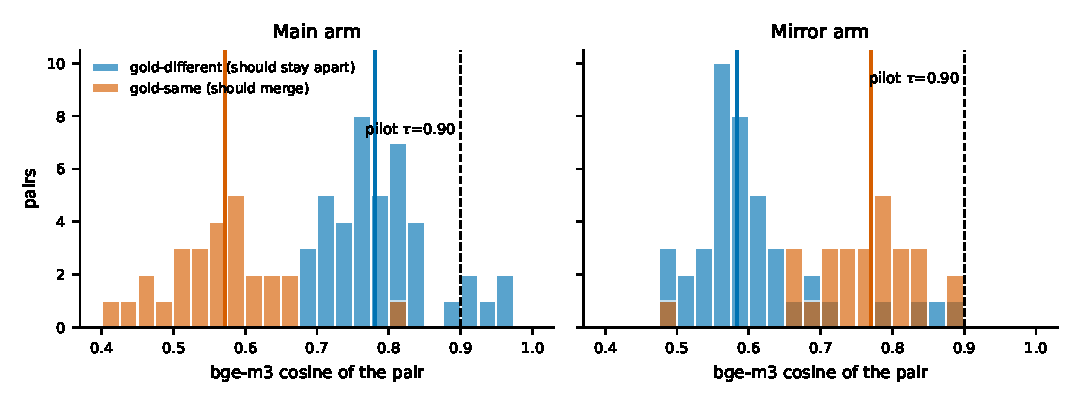
\includegraphics[width=\linewidth]{figures/d_cosine.pdf}
\caption{Raw bge-m3 cosine of the injected pair, by gold relation, per arm (Config D). Solid lines: medians. Dashed: pilot $\tau=0.90$.
All 69 pairs of each arm are drawn.}\label{fig:dcos}
\end{figure}

\paragraph{Mirror arm.} \todo{P1: Config C on the mirror arm: false merges \MirrorCoffHiFCR{} (gate off) $\to$ \MirrorClexHiFCR{} (gate on), missed merges \MirrorCoffHiMCR{} $\to$ \MirrorClexHiMCR{}. The gate helps on both arms.}

\paragraph{QA.} \todo{P1: QA accuracy \MainCoffQA{} (C off) vs \MainClexQA{} (C on); merging affects what the answerer retrieves.}

\subsection{Tier 2 v2: Hindi, Marathi and Gujarati, Configurations A--D}
\label{sec:results-v2}

The v2 arm (frozen as v2.0 before any run) has \VTwoNPairs{} injected pairs, \VTwoNDiff{} gold-different and \VTwoNSame{} gold-same
(Hindi \VTwoNHiDiff{}/\VTwoNHiSame{}, Marathi \VTwoNMrDiff{}/\VTwoNMrSame{}, Gujarati \VTwoNGuDiff{}/\VTwoNGuSame{}, as different/same),
and runs all four configurations with the 7B identity judge for A--C. It is a separate experiment from the v1.0 and mirror arms above
and is not pooled with them. Rates here are at the final memory-record level; the v2 lexicon adds Marathi and Gujarati entries that,
like the Marathi and Gujarati items, are not native-verified. These are provisional development results from one seed.

\begin{table}[t]\centering\small
% GENERATED by paper/tools/make_v2_numbers.py. Do not edit.
\begin{tabular}{llccc}
\toprule
Config & DK-Mem & FCR & MCR & QA \\
\midrule
A (English gloss) & gate off & 11/68 [0.09, 0.27] & 18/58 [0.21, 0.44] & 89/194 \\
A (English gloss) & gate on & 1/68 [0.00, 0.08] & 30/58 [0.39, 0.64] & 94/194 \\
\midrule
B (native-language fact) & gate off & 12/68 [0.10, 0.28] & 5/58 [0.04, 0.19] & 149/194 \\
B (native-language fact) & gate on & 6/68 [0.04, 0.18] & 20/58 [0.24, 0.47] & 152/194 \\
\midrule
C (verbatim) & gate off & 18/68 [0.17, 0.38] & 5/58 [0.04, 0.19] & 163/194 \\
C (verbatim) & gate on & 7/68 [0.05, 0.20] & 20/58 [0.24, 0.47] & 164/194 \\
\midrule
D (cosine, $\tau$=0.90) & gate off & 0/68 [0.00, 0.05] & 56/58 [0.88, 0.99] & 162/194 \\
D (cosine, $\tau$=0.90) & gate on & 0/68 [0.00, 0.05] & 58/58 [0.94, 1.00] & 162/194 \\
\bottomrule
\end{tabular}

\caption{Tier~2 v2 (\VTwoNPairs{} pairs; Hindi, Marathi, Gujarati), one seed, development data, provisional. FCR over the \VTwoNDiff{}
gold-different pairs, MCR over the \VTwoNSame{} gold-same pairs, 95\% Wilson intervals; QA: correct answers over all questions.}
\label{tab:results-v2}
\end{table}

\paragraph{The gate removes the kinship false merges of every LLM host.} With the gate on, false merges fall from \VTwoAOffFCR{} to
\VTwoALexFCR{} (A), \VTwoBOffFCR{} to \VTwoBLexFCR{} (B) and \VTwoCOffFCR{} to \VTwoCLexFCR{} (C). For C the change in the
gold-different merge rate is \VTwoCgateDifferentDiff{} (95\% CI \VTwoCgateDifferentDiffci{}; discordant pairs
\VTwoCgateDifferentDiscordant{}, exact McNemar $p=\VTwoCgateDifferentMcNemar$). On kinship pairs the judge alone merges
\VTwoCOffKinFCR{} gold-different pairs and none with the gate (\VTwoCLexKinFCR{}); A and B also drop to \VTwoALexKinFCR{} and
\VTwoBLexKinFCR{}. The false merges that remain are contextual-qualifier pairs (C: \VTwoCLexQualFCR{}), a class the gate does not cover.
By language, C's false merges go from \VTwoCOffHiFCR{} to \VTwoCLexHiFCR{} in Hindi, \VTwoCOffMrFCR{} to \VTwoCLexMrFCR{} in Marathi
and \VTwoCOffGuFCR{} to \VTwoCLexGuFCR{} in Gujarati; the Marathi and Gujarati cells are small and only indicative.

\paragraph{The cost is missed merges, mostly from register.} Missed merges rise from \VTwoCOffMCR{} to \VTwoCLexMCR{} for C (B:
\VTwoBOffMCR{} to \VTwoBLexMCR{}; A: \VTwoAOffMCR{} to \VTwoALexMCR{}). Most of this comes from gold-same register pairs, in which one
person is addressed with two registers: C misses \VTwoCOffRegMCR{} of them without the gate and \VTwoCLexRegMCR{} with it, because
the gate treats a register difference as evidence of two people while our labelling convention treats a shared vocative as one. In
the pre-registered kinship-only variant, in which register no longer vetoes, C keeps its false merges at \VTwoCLexKOFCR{} and misses
\VTwoCLexKOMCR{} gold-same pairs instead of \VTwoCLexMCR{}. The gold-same kinship pairs that are still blocked (\VTwoCLexKinMCR{}
for C, against \VTwoCOffKinMCR{} without the gate) are lexicon gaps rather than judge errors: one mention names the person without a
kinship term, so only one side carries the feature; a relative is described periphrastically (``mother's sister'' for
\emph{mausi}); \emph{mama ki wife} is tagged as \emph{mama} although it denotes the \emph{mami}; and a spelling variant
(\emph{naani}) is missing.

\paragraph{QA moves little.} QA accuracy is \VTwoCOffQApct\% (C, gate off) and \VTwoCLexQApct\% (gate on); B \VTwoBOffQApct\% and
\VTwoBLexQApct\%; A \VTwoAOffQApct\% and \VTwoALexQApct\%. We did not test these differences; the extra missed merges did not lower
QA accuracy on this benchmark.

\paragraph{The embedding host cannot match the judge at any threshold.} At $\tau=0.90$ Config D merges almost nothing (MCR
\VTwoDOffMCR{}). Over its full frontier (\VTwoDFrontNTaus{} distinct thresholds, none selected), the lowest false consolidation
rate D reaches at C's missed-merge rate is \VTwoDFrontCOffOff\% without the gate and, at the gated C's missed-merge rate,
\VTwoDFrontCLexLex\% with it, against C's own \VTwoCOffFCRpct\% and \VTwoCLexFCRpct\%.
